\documentclass[11pt]{article}
\usepackage[margin=1in]{geometry}
\usepackage{amsmath,amssymb,amsthm}
\usepackage{graphicx}
\usepackage{float}
\usepackage{microtype}
\usepackage[colorlinks=true,linkcolor=blue,citecolor=blue,urlcolor=blue]{hyperref}

\newtheorem{theorem}{Theorem}
\newtheorem{corollary}[theorem]{Corollary}
\newcommand{\CQC}{\mathcal C_{\mathrm{QC}}}
\newcommand{\CCRR}{\mathcal C_{\mathrm{CRR}}}

\title{A Reflection Witness for Unsaturation of\\
\v Ciri\'c Quasi-Contractions}
\author{Solution packet for arXiv:2103.15148, Open Problem 2}
\date{August 11, 2026}

\begin{document}
\maketitle

\begin{center}
\fbox{\parbox{0.92\linewidth}{\textbf{Status.}
Candidate full solution, likely valid.  On every nonzero Banach space the
class of \v Ciri\'c quasi-contractions is unsaturated.  The zero Banach space
is the unique saturated edge case.}}
\end{center}

\section{Source question}

Berinde and P\u acurar ask in Open Problem 2 on printed page 15 of
\cite{BP21} whether the class $\CQC(X)$ of \v Ciri\'c quasi-contractions on a
Banach space $X$ is saturated or unsaturated.  The source statement and its
referenced definition are reproduced below.

\begin{figure}[H]
\centering

\includegraphics[width=\linewidth]{figures/open_problem_crop.png}
\caption{Open Problems 1 and 2 on printed page 15 of \cite{BP21}.}
\end{figure}

\begin{figure}[H]
\centering
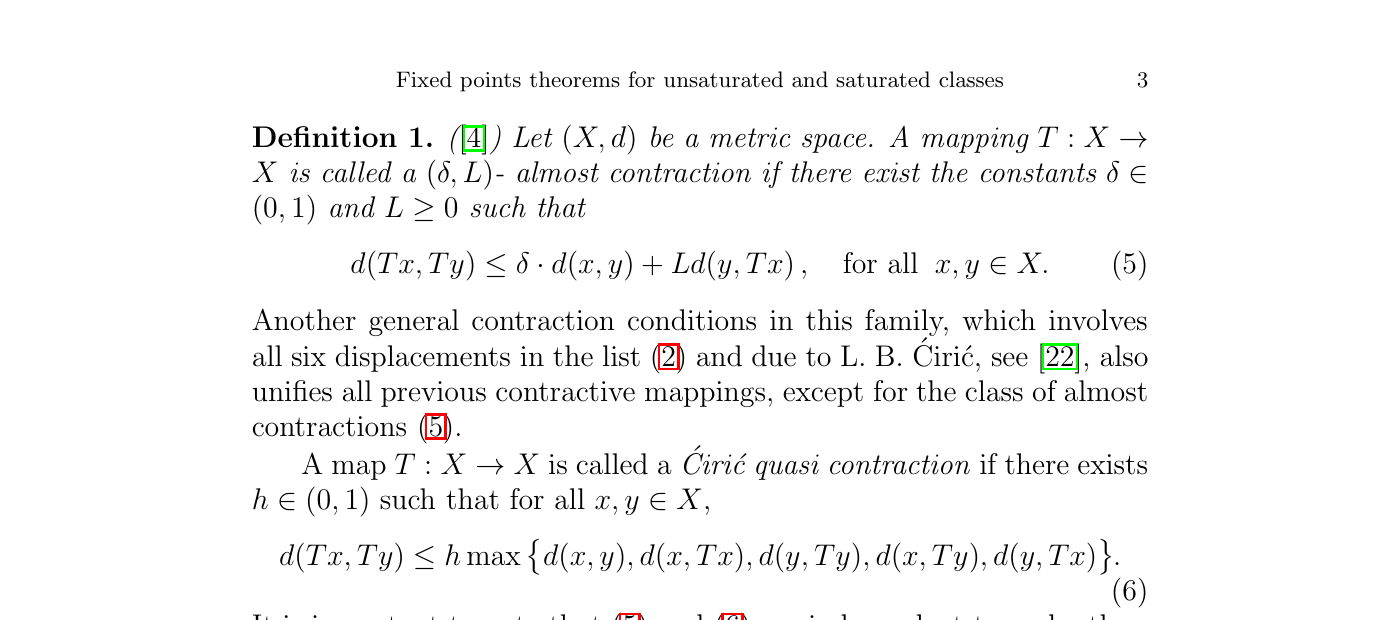
\includegraphics[width=\linewidth]{figures/quasi_contraction_definition_crop.png}
\caption{The defining inequality (6) on printed page 3 of \cite{BP21}.}
\end{figure}

For clarity, a self-map $T:X\to X$ is a \emph{\v Ciri\'c
quasi-contraction} if there is $h\in(0,1)$ such that
\begin{equation}\label{eq:qc}
 \|Tx-Ty\|\le h\max\{\|x-y\|,\|x-Tx\|,\|y-Ty\|,
 \|x-Ty\|,\|y-Tx\|\}
\end{equation}
for every $x,y\in X$.  For $0<\lambda\le1$, its averaged map is
\[
 T_\lambda=(1-\lambda)I+\lambda T.
\]
A map is $\CQC$-enriched if $T_\lambda\in\CQC(X)$ for some such
$\lambda$.  The class is \emph{saturated} when
$\CQC(X)^e=\CQC(X)$ and \emph{unsaturated} when this inclusion is strict.

\section{Idea of the proof}

The averaging operation has a simple extreme behavior that the five-distance
maximum in \eqref{eq:qc} cannot hide.  Take the reflection $R=-I$.  At the
opposite pair $u,-u$, every nonzero term in the maximum equals
$2\|u\|$, exactly the distance between the images.  The strict factor $h<1$
therefore makes the quasi-contraction inequality impossible.  But averaging
$R$ with the identity at $\lambda=1/2$ cancels it completely:
$R_{1/2}=0$, a constant map and hence a quasi-contraction.  Thus one map lies
in the enriched class but not in the original class.

\section{Full answer}

\begin{theorem}\label{thm:main}
Let $X$ be a real or complex Banach space.
\begin{enumerate}
\item If $X\ne\{0\}$, then $\CQC(X)$ is unsaturated.
\item If $X=\{0\}$, then $\CQC(X)$ is saturated.
\end{enumerate}
Consequently, every nonzero Banach space has the same answer to Open Problem
2 of \cite{BP21}: the class is unsaturated.
\end{theorem}

\begin{proof}
Assume first that $X\ne\{0\}$, and let $R=-I_X$.  Choose $u\ne0$ and put
$x=u$, $y=-u$.  Then
\[
 \|Rx-Ry\|=2\|u\|.
\]
For this same pair, the five quantities in the maximum in
\eqref{eq:qc} are, in order,
\[
 2\|u\|,\quad 2\|u\|,\quad 2\|u\|,\quad 0,\quad 0.
\]
If $R$ satisfied \eqref{eq:qc} for some $h<1$, we would therefore have
$2\|u\|\le2h\|u\|$, an impossibility.  Hence $R\notin\CQC(X)$.

On the other hand,
\[
 R_{1/2}=\tfrac12 I_X+\tfrac12(-I_X)=0.
\]
The zero map belongs to $\CQC(X)$: its left-hand side in
\eqref{eq:qc} is zero for all $x,y$, so, for example, $h=1/2$ works.  Thus
$R\in\CQC(X)^e\setminus\CQC(X)$, proving strict inclusion and
unsaturation.

If $X=\{0\}$, there is only one self-map.  It is the zero map, belongs to
$\CQC(X)$, and every one of its averages is itself.  Hence
$\CQC(X)^e=\CQC(X)$.
\end{proof}

The same witness also gives a one-line proof of the source's Open Problem 1,
although that problem was independently answered in later literature
\cite{BP22}.

\begin{corollary}
For every nonzero Banach space $X$, the class $\CCRR(X)$ of
\v Ciri\'c--Reich--Rus contractions is unsaturated; it is saturated on the
zero space.
\end{corollary}

\begin{proof}
For $R=-I$ and $x=u$, $y=-u$, the defining right-hand side is
\[
 a\|x-y\|+b(\|x-Rx\|+\|y-Ry\|)
 =2(a+2b)\|u\|<2\|u\|=\|Rx-Ry\|,
\]
because $a,b\ge0$ and $a+2b<1$.  Thus $R\notin\CCRR(X)$, whereas
$R_{1/2}=0\in\CCRR(X)$.  The zero-space argument is unchanged.
\end{proof}

\section{Verification and limitations}

The proof uses only the definitions.  The critical checks are: $1/2$ is an
allowed averaging parameter; the reflection is a self-map on every real or
complex Banach space; the opposite pair exists exactly when the space is
nonzero; and a constant map satisfies both defining inequalities.  No
completeness property beyond the source's Banach-space hypothesis is used, so
the same result holds on every nonzero normed space.

The theorem classifies saturation only for the source's class
$\CQC(X)$ and its exact enrichment operation.  It does not claim new fixed
point or iteration estimates for the larger enriched class.

\section{Novelty check and review recommendation}

A bounded search through August 11, 2026 used the exact phrases ``\v Ciri\'c
quasi contractions saturated'', ``class of \v Ciri\'c quasi contractions
unsaturated'', and the wording of Open Problem 2, together with searches for
the source title and authors.  It found the source and later general
fixed-point papers, but no paper explicitly answering Open Problem 2.  The
same search found Berinde--P\u acurar's 2022 paper \cite{BP22}, which explicitly
answers Open Problem 1 for \v Ciri\'c--Reich--Rus contractions.  Accordingly,
only Theorem~\ref{thm:main} is presented as the candidate new full result.

Human review is recommended as a high-confidence, low-complexity check.  The
main point to verify is semantic: that Definition 2.1 of \cite{BP21} allows
the self-map $-I_X$ and $\lambda=1/2$ exactly as used above.

\begin{thebibliography}{9}
\bibitem{BP21}
V. Berinde and M. P\u acurar,
\emph{Fixed points theorems for unsaturated and saturated classes of
contractive mappings in Banach spaces},
Symmetry \textbf{13} (2021), 713; arXiv:2103.15148.

\bibitem{BP22}
V. Berinde and M. P\u acurar,
\emph{A new class of unsaturated mappings: \v Ciri\'c--Reich--Rus
contractions},
An. Univ. Ovidius Constan\c ta Ser. Mat. \textbf{30} (2022), no.~3,
37--50, doi:10.2478/auom-2022-0033.
\end{thebibliography}

\end{document}
